\documentclass[
11pt, % The default document font size, options: 10pt, 11pt, 12pt
codirector, % Uncomment to add a codirector to the title page
]{charter} 




% El títulos de la memoria, se usa en la carátula y se puede usar el cualquier lugar del documento con el comando \ttitle
\titulo{Sistema flexible de visión industrial} 

% Nombre del posgrado, se usa en la carátula y se puede usar el cualquier lugar del documento con el comando \degreename
\posgrado{Maestría en Inteligencia Artificial Embebida} 

% Tu nombre, se puede usar el cualquier lugar del documento con el comando \authorname
\autor{Alejandro Virgillo} 

% El nombre del director y co-director, se puede usar el cualquier lugar del documento con el comando \supname y \cosupname y \pertesupname y \pertecosupname
\director{Nombre del Director}
\pertenenciaDirector{pertenencia} 
% FIXME:NO IMPLEMENTADO EL CODIRECTOR ni su pertenencia
\codirector{John Doe} % para que aparezca en la portada se debe descomentar la opción codirector en el documentclass
\pertenenciaCoDirector{FIUBA}

% Nombre del cliente, quien va a aprobar los resultados del proyecto, se puede usar con el comando \clientename y \empclientename
\cliente{A3 Engineering}
\empresaCliente{A3 Engineering}

% Nombre y pertenencia de los jurados, se pueden usar el cualquier lugar del documento con el comando \jurunoname, \jurdosname y \jurtresname y \perteunoname, \pertedosname y \pertetresname.
\juradoUno{Nombre y Apellido (1)}
\pertenenciaJurUno{pertenencia (1)} 
\juradoDos{Nombre y Apellido (2)}
\pertenenciaJurDos{pertenencia (2)}
\juradoTres{Nombre y Apellido (3)}
\pertenenciaJurTres{pertenencia (3)}
 
\fechaINICIO{4 de marzo de 2023}		%Fecha de inicio de la cursada de GdP \fechaInicioName
\fechaFINALPlan{18 de abril de 2023} 	%Fecha de final de cursada de GdP
\fechaFINALTrabajo{4 de octubre de 2023}	%Fecha de defensa pública del trabajo final


\begin{document}

\maketitle
\thispagestyle{empty}
\pagebreak


\thispagestyle{empty}
{\setlength{\parskip}{0pt}
\tableofcontents{}
}
\pagebreak


\section*{Registros de cambios}
\label{sec:registro}


\begin{table}[ht]
\label{tab:registro}
\centering
\begin{tabularx}{\linewidth}{@{}|c|X|c|@{}}
\hline
\rowcolor[HTML]{C0C0C0} 
Revisión & \multicolumn{1}{c|}{\cellcolor[HTML]{C0C0C0}Detalles de los cambios realizados} & Fecha      \\ \hline
0      & Creación del documento                                 &\fechaInicioName \\ \hline
1      & Se completa hasta el punto 5 y parte del punto 6       & 29 de marzo de 2023 \\ \hline
2      & Se completa el plan									& 1 de abril de 2023 \\ \hline
%		  Se puede agregar algo más \newline
%		  En distintas líneas \newline
%		  Así                                                    & dd/mm/aaaa \\ \hline
%3      & Se completa hasta el punto 11 inclusive                & dd/mm/aaaa \\ \hline
%4      & Se completa el plan	                                 & dd/mm/aaaa \\ \hline
\end{tabularx}
\end{table}

\pagebreak



\section*{Acta de constitución del proyecto}
\label{sec:acta}

\begin{flushright}
Buenos Aires, \fechaInicioName
\end{flushright}

\vspace{2cm}

Por medio de la presente se acuerda con el Ing. \authorname\hspace{1px} que su Trabajo Final de la \degreename\hspace{1px} se titulará ``\ttitle'', consistirá esencialmente en la implementación de una interfaz y elementos de visión de máquina que permitan programar verificaciones de calidad en procesos industriales, y tendrá un presupuesto preliminar estimado de 570 h de trabajo y U\$D 7565, con fecha de inicio \fechaInicioName\hspace{1px} y fecha de presentación pública \fechaFinalName.

Se adjunta a esta acta la planificación inicial.

\vfill

% Esta parte se construye sola con la información que hayan cargado en el preámbulo del documento y no debe modificarla
\begin{table}[ht]
\centering
\begin{tabular}{ccc}
\begin{tabular}[c]{@{}c@{}}Dr. Ing. Ariel Lutenberg \\ Director posgrado FIUBA\end{tabular} & \hspace{2cm} & \begin{tabular}[c]{@{}c@{}}\clientename \\ \empclientename \end{tabular} \vspace{2.5cm} \\ 
\multicolumn{3}{c}{\begin{tabular}[c]{@{}c@{}} \supname \\ Director del Trabajo Final\end{tabular}} \vspace{2.5cm} \\
%\begin{tabular}[c]{@{}c@{}}\jurunoname \\ Jurado del Trabajo Final\end{tabular}     &  & \begin{tabular}[c]{@{}c@{}}\jurdosname\\ Jurado del Trabajo Final\end{tabular}  \vspace{2.5cm}  \\
%\multicolumn{3}{c}{\begin{tabular}[c]{@{}c@{}} \jurtresname\\ Jurado del Trabajo Final\end{tabular}} \vspace{.5cm}                                                                     
\end{tabular}
\end{table}




\section{1. Descripción técnica-conceptual del proyecto a realizar}
\label{sec:descripcion}

En la actualidad, las empresas industriales suelen realizar inspecciones en sus líneas de producción para garantizar la calidad de sus productos. Una de las técnicas más empleadas es la inspección visual, que permite determinar si una pieza cuenta con defectos y realizar acciones acorde. Con el avance de la tecnología este proceso se ha logrado automatizar con el uso de sistemas de visión. Estos permiten realizar revisiones más precisas que las que puede hacer una persona y sobre el 100\% de las piezas.

Un sistema de visión industrial está conformado por cámaras, lentes, elementos de iluminación y dispositivos de procesamiento. Para trabajar dentro de una línea de manufactura automática tienen la capacidad de comunicarse con los controladores centrales del proceso, generalmente del tipo PLC (\textit{Programmable Logic Controller}), a través de señales discretas o protocolos de comunicación industrial. 

En el mercado existe una gran oferta de sistemas de visión industriales que ofrecen interfaces de programación simples con diversas herramientas incorporadas para facilitar los trabajos de inspección. Suelen ser flexibles a la hora de seleccionar componentes de iluminación, lentes y cámaras, y tienen la capacidad de comunicarse con controladores industriales a través de señales discretas y diferentes protocolos de comunicación. Su problema radica en sus altos costos, que pueden ser prohibitivos para muchas aplicaciones.

En lo que refiere al procesamiento de imágenes, los sistemas que se comercializan cuentan con un gran número de filtros, herramientas de detección y algoritmos de aprendizaje que se eligen según el problema a resolver. Las mismas consideraciones deben tenerse en cuenta a la hora de seleccionar el sensor, el lente y los elementos de iluminación, y también su disposición en el espacio. En general, este tipo de problemas suele ser complejo y requerir de un alto grado de ensayos previo a alcanzar el resultado deseado.

En este proyecto se busca conseguir un sistema de visión que permita procesar imágenes para determinar si, en un proceso industrial de producción, ciertas piezas con las que se trabaja cumplen con algunas restricciones específicas de calidad. Este debe ser de bajo costo y poder controlar un sistema de iluminación, tomar información de una cámara, envíar señales a un PLC y ofrecer una interfaz de usuario para su programación y monitoreo. 

En la Figura \ref{fig:diagBloques} se muestra un diagrama en bloques del sistema a implementar. El proyecto abarca el diseño del software de la parte que aparece denominada como controlador y su interacción con los demás bloques. También se incluye el diseño y fabricación del bloque que se denomina Adaptación IO, que corresponde a un circuito eléctrico de acondicionamiento de señales. La selección de periféricos y de interfaz física es parte del proyecto. 

\begin{figure}[htpb]
\centering 
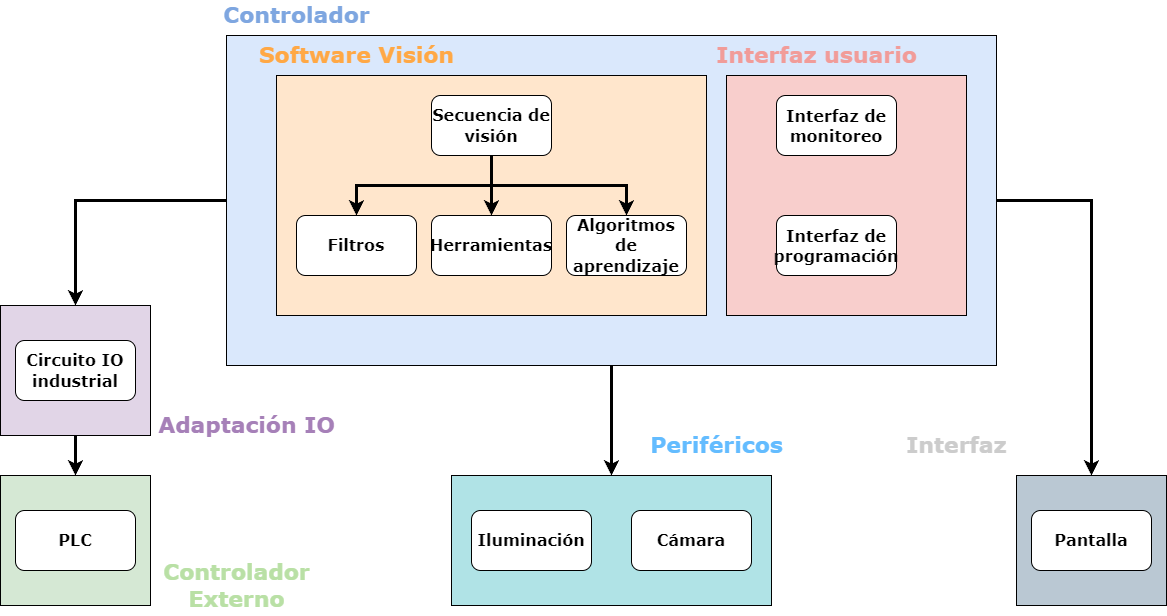
\includegraphics[width=.8\textwidth]{./Figuras/TPF_CEIA_diagrama_bloques.png}
\caption{Diagrama en bloques del sistema}
\label{fig:diagBloques}
\end{figure}

Se plantea usar una placa controladora Raspberry Pi, que es de fácil acceso y cuenta con muchas herramientas para conectar cámaras y pantallas. Sobre esta se busca diseñar y construir otra plaqueta que aísle eléctricamente y transforme los niveles de tensión de las señales discretas para poder interactuar con un PLC.

El proyecto también involucra el diseño e implementación de una interfaz gráfica, a través de la cual se puedan programar las distintas herramientas de visión, los filtros de imagen, los algoritmos de reconocimiento y el envío de señales.

El proyecto se encará como un trabajo personal junto a la organización A3 Engineering. Mediante un acuerdo con la empresa Cambre ICyFSA, se plantea ensayar el producto obtenido en algunos de sus procesos industriales para controlar la calidad de los productos según las especificaciones correspondientes.

En el aspecto comercial, el producto a obtener se planifica para poder ser vendido en el mercado, para tareas de automatización en procesos industriales. En la Figura \ref{fig:canvas} se presenta un esquema de modelo canvas del negocio. Como se puede observar, la propuesta de valor es ofrecer un producto que permita realizar automatizaciones, principalmente a pequeñas y medianas empresas para las cuales la inversión en sistemas convencionales de visión resulta de riesgo elevado.

\begin{figure}[htpb]
\centering 
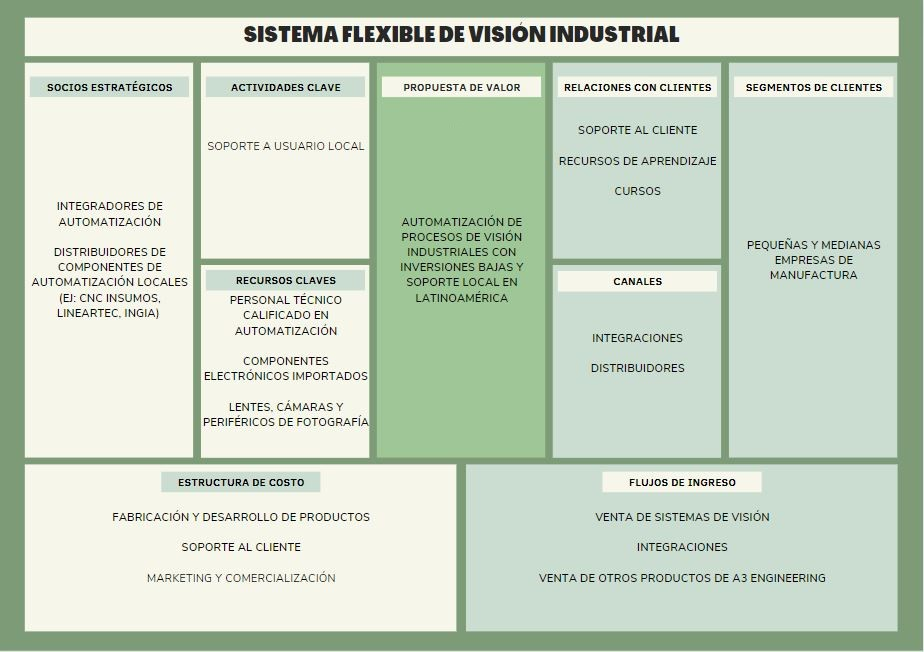
\includegraphics[width=1\textwidth]{./Figuras/modelo_canvas.JPG}
\caption{Modelo canvas del negocio}
\label{fig:canvas}
\end{figure}

Para alcanzar la propuesta de valor se busca alcanzar un sistema enfocado en resolver problemáticas simples, a un costo que permita una recuperación de la inversión más rápida y con soporte local en sudamérica, donde la oferta actual es escasa.

\section{2. Identificación y análisis de los interesados}
\label{sec:interesados}

\begin{table}[ht]
%\caption{Identificación de los interesados}
%\label{tab:interesados}
\begin{tabularx}{\linewidth}{@{}|l|X|X|l|@{}}
\hline
\rowcolor[HTML]{C0C0C0} 
Rol           & Nombre y Apellido & Organización 	& Puesto 	\\ \hline
Auspiciante   & Alejandro Virgillo & A3 Engineering	& Líder de proyecto	 \\ \hline
Cliente       & \supname & \pertesupname	&  Director de proyecto \\ \hline
Impulsor      & Sector de Automatización & Cambre             	& -       	\\ \hline
Responsable   & Alejandro Virgillo  & FIUBA        	& Alumno 	\\ \hline
Colaboradores & Equipo de Ingeniería & Cambre      	& Ingenieros   	\\ \hline
Orientador    & \supname	      & \pertesupname 	& Director Trabajo final \\ \hline
Usuario final & Equipo de Armado  & Cambre         	& Operarios       	\\ \hline
Usuario final & Equipo de Automatización  & Cambre  & Técnicos       	\\ \hline
\end{tabularx}
\end{table}

\begin{itemize}
	\item Colaboradores: El equipo de ingeniería de Cambre puede dar lineamientos de problemas que tengan hoy con sus sistemas de visión en planta.
	\item Orientador: \supname trabajó extensamente con sistemas de visión, es una persona a la que se le puede preguntar sobre dudas que pueda haber en el desarrollo.
	\item Usuario final: Es importante ir ensayando los prototipos con los usuarios finales para obtener feedback del dispositivo.
\end{itemize}

\section{3. Propósito del proyecto}
\label{sec:proposito}

El propósito de este proyecto es obtener un sistema de visión flexible con una interfaz de programación básica que ofrezca algunas de las herramientas más comunes presentes en sistemas comerciales, pero a un costo significativamente menor.

\section{4. Alcance del proyecto}
\label{sec:alcance}


El proyecto incluye:

\begin{itemize}
	\item Una interfaz de usuario para configurar programas de visión.
	\item La implementación de las herramientas de software de visión.
	\item El diseño de una plaqueta para adaptación de señales discretas.
	\item El desarrollo de un gabinete que abarque al sistema.
	\item El ensayo en planta del sistema.
\end{itemize}

El proyecto no incluye:

\begin{itemize}
	\item La implementación de protocolos de comunicación industrial.
	\item El desarrollo de los algorítmos de visión.	
	\item La implementación final en planta.
\end{itemize}

\section{5. Supuestos del proyecto}
\label{sec:supuestos}

Para el desarrollo del proyecto se supone que:

\begin{itemize}
	\item El dinero disponible será suficiente para la adquisición de los materiales requeridos.
	\item Habrá stock de los componentes del sistema y no habrá problemas de importación.
	\item Las demoras para obtener los componentes no serán excesivas.
	\item La relación con la empresa Cambre se mantendrá durante el transcurso del proyecto.
\end{itemize}

\section{6. Requerimientos}
\label{sec:requerimientos}

\newcommand{\leadingZeroes}[1]{%
\ifnum #1<100{0}\fi%
\ifnum #1<10{0}\fi%
#1}
%
\newcounter{REQ}
%
\newcommand{\REQ}{%
\stepcounter{REQ}%
\textbf{[SFVI-REQ{\leadingZeroes{\theREQ}]}}}
%

\begin{enumerate}

	\item \textbf{Requerimientos generales:}
	\begin{enumerate}
		\item El sistema debe utilizar una Raspberry Pi 4. \REQ
		\item El software de visión y la interfaz gráfica deben ser procesados por la Raspberry Pi. \REQ
		\item La Raspberry Pi debe utilizar el sistema operativo Raspbian. \REQ
		\item El sistema debe alimentarse con 24 V de corriente contínua. \REQ
		\item El tiempo máximo de una inspección debe ser menor a 3 segundos. \REQ	
	\end{enumerate}
	
	\item \textbf{Requerimientos de IO:}
	\begin{enumerate}
		\item El sistema debe contar con una plaqueta de adaptación de señales discretas. \REQ
		\item Las señales discretas del sistema deben ser las disponibles en la Raspberry Pi. \REQ
		\item La plaqueta de adaptación de señales debe aislar eléctricamente las señales al menos a 3 KV, mediante el uso de optoacopladores. \REQ
		\item Las señales adaptadas deben ser del tipo PNP. \REQ
		\item La alimentación de las señales debe poder separarse de la alimentación del sistema. \REQ
		\item La alimentación de las señales debe poder estar entre 5 a 48 V de corriente contínua. \REQ
		\item El sistema debe contar con las siguientes señales de entrada: disparador, selección de programa. \REQ
		\item El sistema debe contar con las siguientes señales de salida: Inspección OK, encendido de iluminación, Inspección NO-OK, número de herramienta NO-OK. \REQ
	\end{enumerate}
	
	\item \textbf{Requerimientos de software:}
	\begin{enumerate}
		\item El software debe tener un control de versiones. \REQ
		\item El sistema debe contar con una interfaz gráfica. \REQ
		\item El código del sistema debe realizarse en lenguaje Python. \REQ
		\item El sistema puede utilizar librerias de código abierto como OpenCV. \REQ
	\end{enumerate}
	
	\item \textbf{Requerimientos de visión:}
	\begin{enumerate}
		\item El sistema debe poder controlar la adquisición de imágenes. \REQ
		\item Se debe poder configurar para la adquisición el tiempo de exposición y la ganancia, en caso de que el hardware lo permita. \REQ
		\item Se debe poder configurar una señal de entrada como disparador y una señal de salida como flash. Ambas deben tener retardos configurables. \REQ
		\item Se deben poder aplicar hasta 5 filtros a la imagen adquirida. \REQ
		\item Se deben poder seleccionar y configurar, por lo menos, los siguientes filtros: difuminación, difuminación gaussiana, dilatación, erosión, sobel. \REQ
		\item Se debe poder seleccionar y configurar el ecualizado por histograma de las imágenes. \REQ
		\item El sistema debe contar con herramientas para reconocimiento de bordes y líneas. \REQ
		\item El sistema debe permitir realizar mediciones lineales entre bordes y líneas reconocidos. \REQ
		\item El sistema debe contar con un módulo de aprendizaje profundo para inspecciones de calidad. \REQ
		\item El sistema debe contar con un módulo de reconocimiento de patrón. \REQ
		\item El sistema debe ser poder reconocer el patrón con variaciones de rotación, aspecto y tamaño. El rango permitido para cada uno debe poder configurarse. \REQ
		\item El sistema debe contar con herramientas lógicas para configuración de inspecciones. \REQ
	\end{enumerate}
	
	\item \textbf{Requerimientos de interfaz gráfica:}
	\begin{enumerate}
		\item El sistema debe contar con 2 modos de funcionamiento: programación y operación. \REQ
		\item La interfaz gráfica debe permitir el paso de un modo de funcionamiento a otro. \REQ
		\item El modo de programación debe solo poder accederse mediante el ingreso de una contraseña. \REQ
		\item La interfaz debe permitir configurar la adquisición de imágenes. \REQ
		\item La interfaz debe permitir distintos programas de visión. \REQ
		\item La interfaz debe permitir configurar la estructura de los programas de visión. \REQ
		\item La interfaz debe permitir configurar cada una de las herramientas disponibles por el módulo de visión. \REQ
		\item En modo operación, el sistema debe mostrar la última inspección realizada y el resultado de las distintas herramientas. \REQ
		\item En modo operación, el sistema debe mostrar métricas de inspecciones totales y porcentaje de inspecciones correctas. \REQ
	\end{enumerate}
	
\end{enumerate}


\section{7. Historias de usuarios (\textit{Product backlog})}
\label{sec:backlog}

En esta sección se enuncian las historias de usuario, cada una de ellas llevará un puntaje según 3 aspectos:

\begin{itemize}

	\item Dificultad: Cantidad de trabajo a realizar.
	\item Complejidad: Complejidad de trabajo a realizar.
	\item Riesgo: Incertidumbre del trabajo a realizar.

\end{itemize}

Se utilizará una escala siguiendo la serie de Fibonacci, donde un número mayor implica mayor costo. Si la suma de los 3 componentes no da un número de la serie, se eligirá el próximo más cercano.

\begin{enumerate}

	\item Como operario quiero detectar la presencia de errores para reportarlo a mi supervisor.
	\begin{itemize}
		\item D: 8.
		\item C: 5.
		\item R: 3.
		\item Total: 21.
	\end{itemize}

	\item Como operario quiero una interfaz de usuario simple para evitar cometer errores.
	\begin{itemize}
		\item D: 3.
		\item C: 3.
		\item R: 1.
		\item Total: 7.
	\end{itemize}
	
	\item Como operario de mantenimiento quiero detectar los problemas del sistema para repararlos rápidamente.
	\begin{itemize}
		\item D: 5.
		\item C: 5.
		\item R: 3.
		\item Total: 13.
	\end{itemize}
	
	\item Como desarrollador quiero tener acceso a las distintas herramientas del sistema de visión de una forma ordenada y poder configurarlas fácilmente.
	\begin{itemize}
		\item D: 5.
		\item C: 5.
		\item R: 3.
		\item Total: 13.
	\end{itemize}	
	
	\item Como gerente de planta quiero saber las métricas de calidad y entender dónde están los problemas que reducen la productividad por descarte de piezas malas.
	\begin{itemize}
		\item D: 3.
		\item C: 3.
		\item R: 5.
		\item Total: 11.
	\end{itemize}	
	
\end{enumerate}

\section{8. Entregables principales del proyecto}
\label{sec:entregables}

Los entregables del proyecto son:

\begin{itemize}

	\item Prototipo del sistema.
	\item Ejemplo de implementación.
	\item Manual de uso.
	\item Diagrama de circuitos esquemáticos.
	\item Archivos de fabricación de PCB.
	\item Planos y medidas dimensionales del sistema.
	\item Informe final.

\end{itemize}

\section{9. Desglose del trabajo en tareas}
\label{sec:wbs}

A continuación se enumeran las tareas del proyecto y se detalla su carga horaria:

\begin{enumerate}
	\item \textbf{Planificación y gestión del proyecto (70 hs):}
	\begin{enumerate}
		\item Realizar el plan de trabajo (10 hs)
		\item Reuniones con director (30 hs)
		\item Realizar informe de avance (10 hs)
		\item Confección de memoria de trabajo (40 hs)
		\item Presentación y defensa de trabajo (10 hs)
	\end{enumerate}
	
	\item \textbf{Tareas de investigación (95 hs):}
	\begin{enumerate}
		\item Búsqueda de soluciones similares (10 hs)
		\item Estudiar prestaciones Raspberry Pi (10 hs)
		\item Selección y adquisición de componentes de desarrollo (20 hs)
		\item Estudiar bibliografía de visión (40 hs)
		\item Recopilar hojas de datos (5 hs.)
		\item Búsqueda y estudio de librerías de software (20 hs)
	\end{enumerate}
	
	\item \textbf{Desarrollo de software (200 hs):}
	\begin{enumerate}
		\item Instalación de sistema operativo y librerías (10 hs)
		\item Pruebas de librerías y herramientas de visión (20 hs)
		\item Desarrollo de módulo de visión (60 hs)
		\item Desarrollo de módulo de aprendizaje profundo (30 hs)
		\item Desarrollo de interfaz gráfica (40 hs)
		\item Desarrollo de aplicación (40 hs)
	\end{enumerate}	
	
	\textbf{\item Desarrollo de Hardware (45 hs):}
	\begin{enumerate}
		\item Diseño de circuitos eléctricos (15 hs)
		\item Diseño de PCB (15 hs)
		\item Elaboración de archivos de fabricación (15 hs)
	\end{enumerate}
	
	\textbf{\item Fabricación (60 hs):}
	\begin{enumerate}
		\item Compra de componentes electrónicos (15 hs)
		\item Fabricación de PCB (5 hs)
		\item Ensamble de PCB (10 hs)
		\item Diseño y fabricación de gabinete (30 hs)
	\end{enumerate}
	
	\textbf{\item Ensayos e implementación(100 hs):}
	\begin{enumerate}
		\item Pruebas eléctricas (10 hs)
		\item Ensayo de interfaz de usuario (20 hs)
		\item Prueba de aplicación (20 hs)
		\item Optimización y búsqueda de errores (20 hs)
		\item Pruebas de implementación en planta (30 hs)
	\end{enumerate}
\end{enumerate}	

\section{10. Diagrama de Activity On Node}
\label{sec:AoN}

La Figura \ref{fig:AoN} muestra las actividades del proyecto desglosadas en un diagrama de Activity on Node. Se puede ver la secuencia que conecta las distintas acciones. El tiempo que se muestra representa horas de trabajo.

\begin{figure}[htpb]
	\centering 
	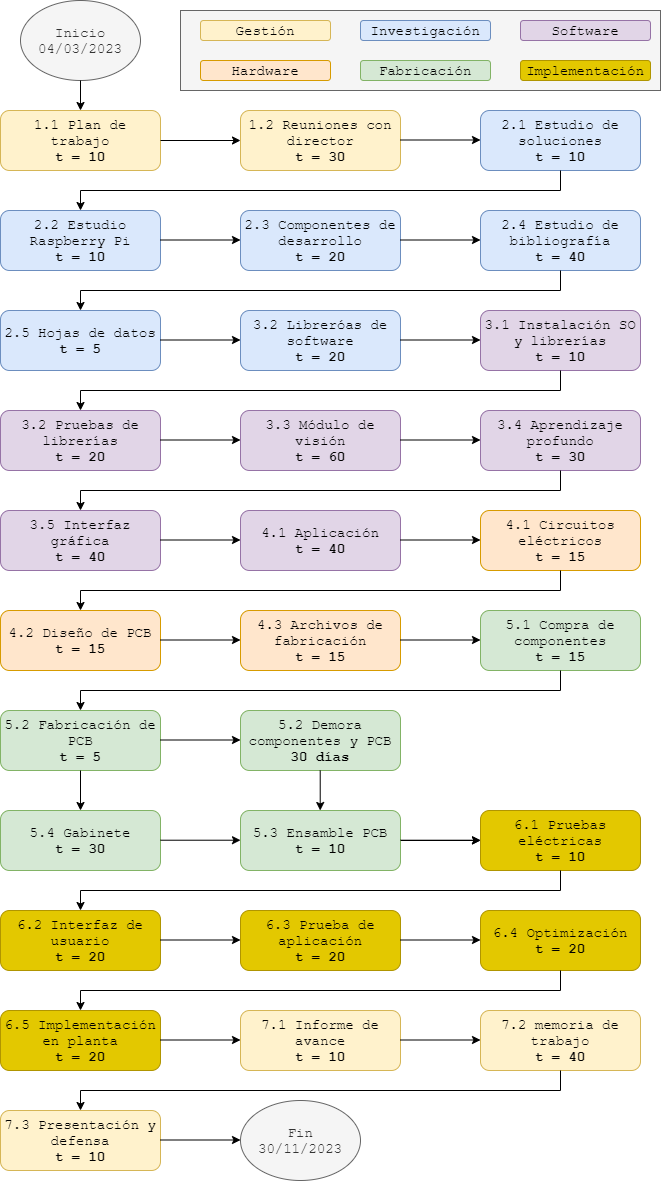
\includegraphics[width=.8\textwidth]{./Figuras/AoN.png}
	\caption{Diagrama de \textit{Activity on Node}}
	\label{fig:AoN}
\end{figure}

\section{11. Diagrama de Gantt}
\label{sec:gantt}

En la figura \ref{fig:WBSGantt} se muestra el esquema de desglose de trabajo y en la figura \ref{fig:diagGantt}, el diagrama de gantt del proyecto.

\begin{figure}[htpb]
\centering 
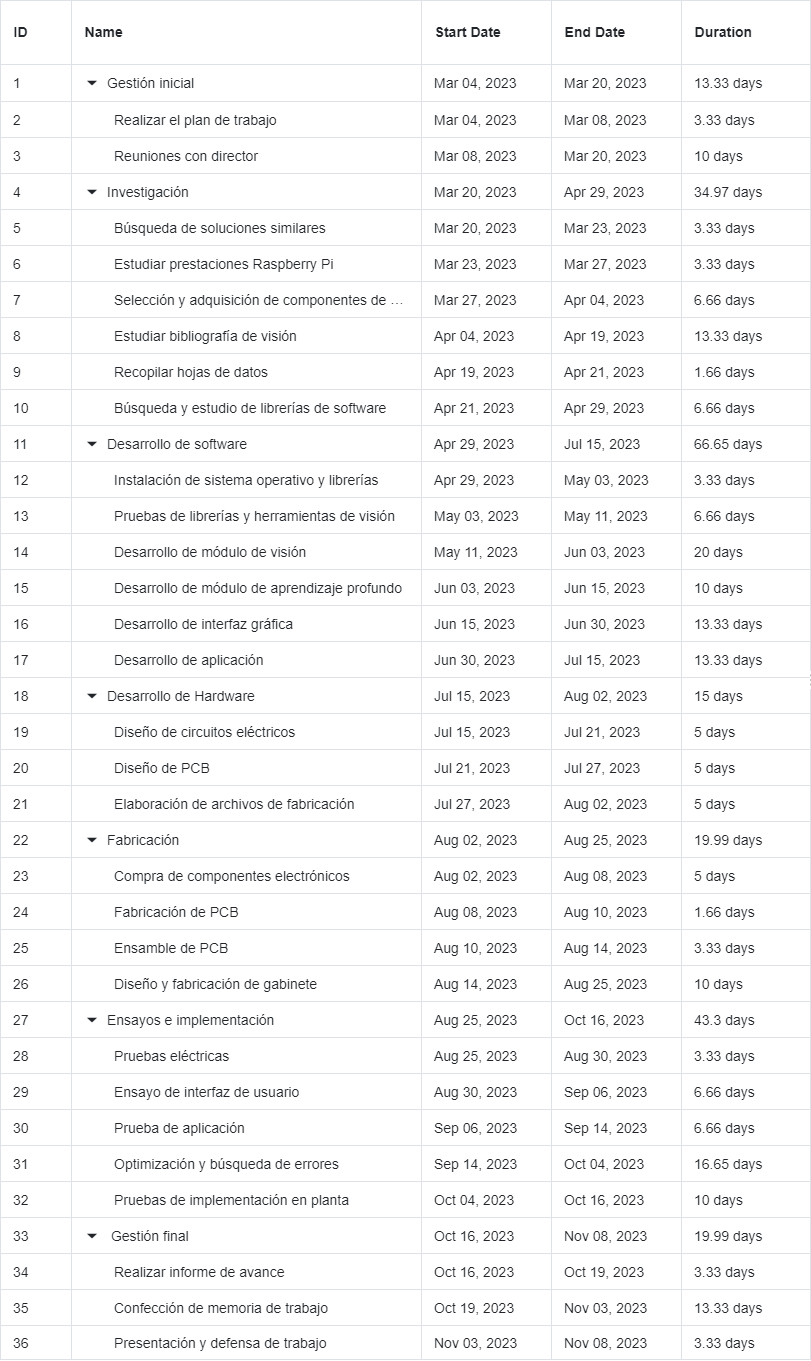
\includegraphics[height=.9\textheight]{./Figuras/wbs.png}
\caption{Desglose de trabajo}
\label{fig:WBSGantt}
\end{figure}

\begin{landscape}
\begin{figure}[htpb]
\centering 
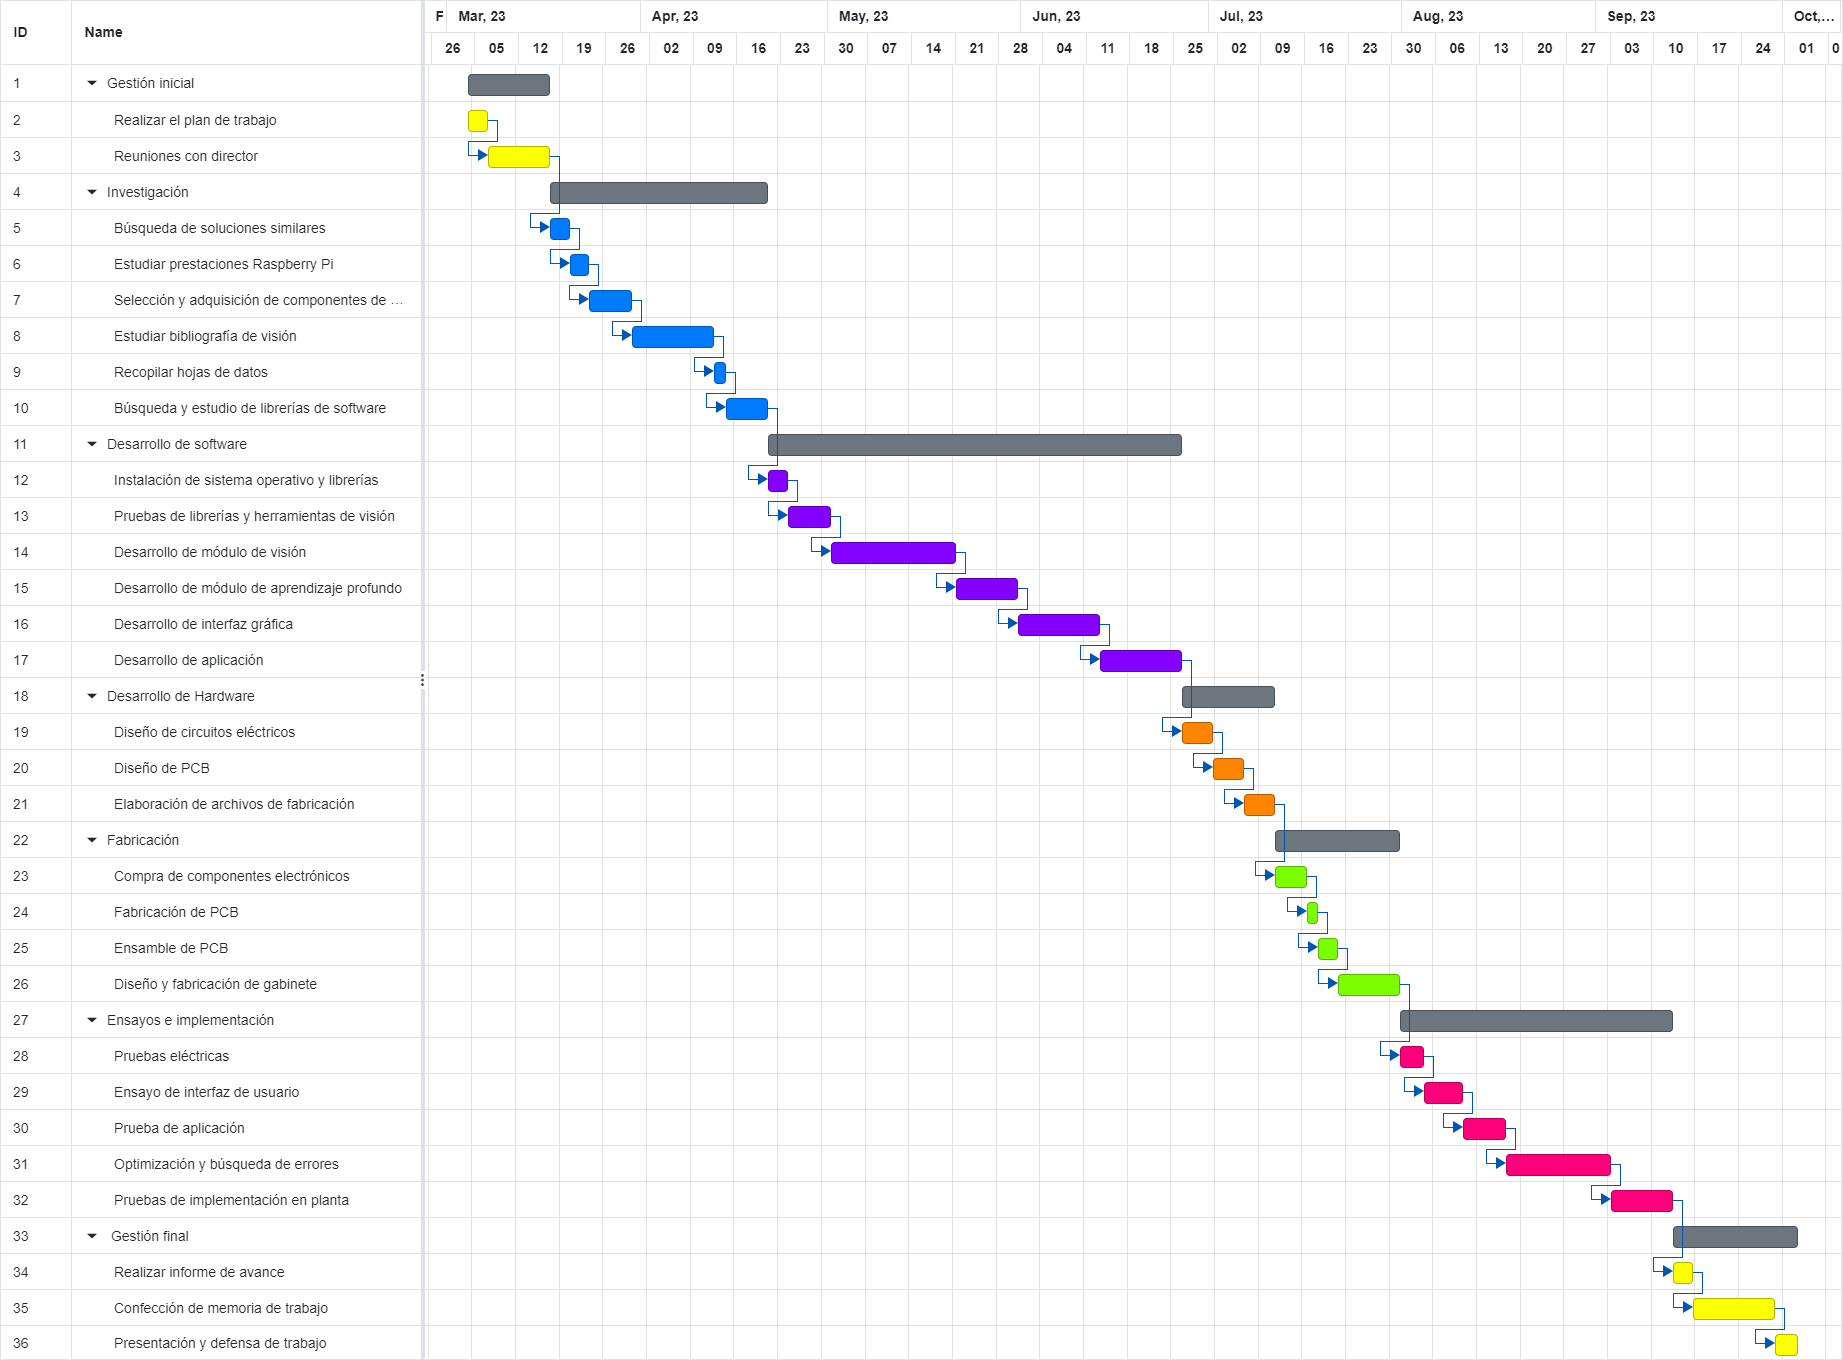
\includegraphics[height=0.9\textheight]{./Figuras/gantt.png}
\caption{Diagrama de Gantt}
\label{fig:diagGantt}
\end{figure}
\end{landscape}

\section{12. Presupuesto detallado del proyecto}
\label{sec:presupuesto}

En el cuadro \ref{tab:costosProyecto} se detallan los costos del proyecto. Se aclara que la cotización del dólar estadounidense (U\$D) al día de la fecha (1 de abril de 2023) es 208.39 AR\$ (pesos argentinos).

\begin{table}[htpb]
\centering
\begin{tabularx}{\linewidth}{@{}|X|c|r|r|@{}}
\hline
\rowcolor[HTML]{C0C0C0} 
\multicolumn{4}{|c|}{\cellcolor[HTML]{C0C0C0}COSTOS DIRECTOS} \\ \hline
\rowcolor[HTML]{C0C0C0} 
Descripción &
  \multicolumn{1}{c|}{\cellcolor[HTML]{C0C0C0}Cantidad} &
  \multicolumn{1}{c|}{\cellcolor[HTML]{C0C0C0}Valor unitario} &
  \multicolumn{1}{c|}{\cellcolor[HTML]{C0C0C0}Valor total} \\ \hline
Horas de ingeniería &
  \multicolumn{1}{c|}{570} &
  \multicolumn{1}{c|}{10 U\$D} &
  \multicolumn{1}{c|}{5700 U\$D} \\ \hline
  
Dispositivos de testing &
  \multicolumn{1}{c|}{1} &
  \multicolumn{1}{c|}{400 U\$D} &
  \multicolumn{1}{c|}{400 U\$D} \\ \hline
  
Componentes electrónicos &
  \multicolumn{1}{c|}{1} &
  \multicolumn{1}{c|}{200 U\$D} &
  \multicolumn{1}{c|}{200 U\$D} \\ \hline
  
Placas PCB &
  \multicolumn{1}{c|}{1} &
  \multicolumn{1}{c|}{100 U\$D} &
  \multicolumn{1}{c|}{100 U\$D} \\ \hline  
  
Gabinete &
  \multicolumn{1}{c|}{1} &
  \multicolumn{1}{c|}{50 U\$D} &
  \multicolumn{1}{c|}{50 U\$D} \\ \hline  

Implementación en planta &
  \multicolumn{1}{c|}{1} &
  \multicolumn{1}{c|}{500 U\$D} &
  \multicolumn{1}{c|}{500 U\$D} \\ \hline 

\multicolumn{3}{|c|}{SUBTOTAL} &
  \multicolumn{1}{c|}{6950 U\$D} \\ \hline
\rowcolor[HTML]{C0C0C0} 
\multicolumn{4}{|c|}{\cellcolor[HTML]{C0C0C0}COSTOS INDIRECTOS} \\ \hline
\rowcolor[HTML]{C0C0C0} 
Descripción &
  \multicolumn{1}{c|}{\cellcolor[HTML]{C0C0C0}Cantidad} &
  \multicolumn{1}{c|}{\cellcolor[HTML]{C0C0C0}Valor unitario} &
  \multicolumn{1}{c|}{\cellcolor[HTML]{C0C0C0}Valor total} \\ \hline
  
Horas de administración &
  \multicolumn{1}{c|}{50} &
  \multicolumn{1}{c|}{5 U\$D} &
  \multicolumn{1}{c|}{250 U\$D} \\ \hline 

Horas de uso de PC &
  \multicolumn{1}{c|}{570} &
  \multicolumn{1}{c|}{0.5 U\$D} &
  \multicolumn{1}{c|}{285 U\$D} \\ \hline 
  
Horas de uso de máquinas &
  \multicolumn{1}{c|}{40} &
  \multicolumn{1}{c|}{2 U\$D} &
  \multicolumn{1}{c|}{80 U\$D} \\ \hline 

\multicolumn{3}{|c|}{SUBTOTAL} &
  \multicolumn{1}{c|}{615 U\$D} \\ \hline
\rowcolor[HTML]{C0C0C0}
\multicolumn{3}{|c|}{TOTAL} &
\multicolumn{1}{c|}{7565 U\$D}
   \\ \hline
\end{tabularx}%
\caption{Costos del proyecto}
\label{tab:costosProyecto}
\end{table}

\section{13. Gestión de riesgos}
\label{sec:riesgos}

a) Riesgos identificados:

Riesgo 1: No habrá stock de los componentes necesarios.
\begin{itemize}
	\item Severidad (S): 8. Sin los componentes no se podrá ensayar ni finalizar el proyecto.
	\item Probabilidad de ocurrencia (O): 5. Actualmente, existe una escasez general de componentes electrónicos en el mercado, aunque los necesarios son de amplio uso. 
\end{itemize}   

Riesgo 2: El fabricante de PCBs tendrá demoras excesivas o problemas con la fabricación.
\begin{itemize}
	\item Severidad (S): 6. Sin la placa, solo se podrá hacer un prototipo provisorio para las IO. No podrá completarse el proyecto en tiempo de forma satisfactoria
	\item Ocurrencia (O): 2. Hay varios fabricantes y con los que se trabajó previamente nunca hubo inconvenientes.
\end{itemize}

Riesgo 3: Se perderá la relación actual con la empresa Cambre.
\begin{itemize}
	\item Severidad (S): 5. Se complicaría realizar testeos en planta, así como algunas facilidades para la obtención de los componentes.
	\item Ocurrencia (O): 2. Actualmente, la relación es muy buena.
\end{itemize}

Riesgo 4: Aparecerán trabas políticas en materia aduanera, o complicaciones económicas en Argentina.
\begin{itemize}
	\item Severidad (S): 7. Se dificultaría conseguir los componentes y las PCB.
	\item Ocurrencia (O): 5. La inestabilidad política actual puede generar problemas.
\end{itemize}

b) Tabla de gestión de riesgos (El RPN se calcula como RPN=SxO): 

\begin{table}[htpb]
\centering
\begin{tabular}{|c|c|c|c|c|c|c|}
\hline
\rowcolor[HTML]{C0C0C0} 
Riesgo & Severidad & Ocurrencia & RPN & Severidad* & Ocurrencia* & RPN* \\ \hline
    1  & 8  & 5  &  40   &  6  & 4   & 24     \\ \hline
    2  & 6  & 2  &  12   &  -  &  -  & -    \\ \hline
    3  & 5  & 2  &  10   &  -  &  -  & -     \\ \hline
    4  & 7  & 5  &  35   &  5  &  5  & 25     \\ \hline
\end{tabular}%
\end{table}

Criterio adoptado: 
Se tomarán medidas de mitigación en los riesgos cuyos números de RPN sean mayores a 30.

Nota: los valores marcados con (*) en la tabla corresponden luego de haber aplicado la mitigación.

c) Plan de mitigación de los riesgos que originalmente excedían el RPN máximo establecido:
 
Riesgo 1: Se buscará determinar lo antes posible los componentes a usar y encargarlos de inmediato.
\begin{itemize}
  \item Severidad (S): 6. La severidad es menor ya que el problema se afrontaría antes, permitiendo no atrasarse o seleccionar otros componentes similares y diseñar a partir de estos.
  \item Probabilidad de ocurrencia (O): 4. Si bien puede que no haya stock, se tendrá un mayor margen de tiempo en el cual se pueden conseguir los componentes.
\end{itemize}
  
Riesgo 4: Similar al plan del Riesgo 1, se buscará determinar los componentes lo antes posible y encargarlos.
\begin{itemize}
	\item Severidad (S): 5. Teniendo los componentes en mano, el proyecto tiene menos retrasos debido a un cierre.
  \item Probabilidad de ocurrencia (O): 5. La posibilidad de que ocurra un cierre se mantiene igual, pero la posibilidad de no tener los componentes disminuye.
\end{itemize}

\section{14. Gestión de la calidad}
\label{sec:calidad}

Para cada uno de los requerimientos del proyecto se enuncia el procedimiento de verificación y validación:

\setcounter{REQ}{0}
\begin{itemize} 

	\item \REQ El sistema debe utilizar una Raspberry Pi 4:
	\begin{itemize}
		\item Verificación: Se comprobará el componente empleado.
		\item Validación: Se comprobará la conformación del sistema.
	\end{itemize}
	
	\item \REQ El software de visión y la interfaz gráfica deben ser procesados por la Raspberry Pi:
	\begin{itemize}
		\item Verificación: Se comprobará el software empleado.
		\item Validación: Se comprobará la conformación del sistema.
	\end{itemize}
	
	\item \REQ La Raspberry Pi debe utilizar el sistema operativo Raspbian:
	\begin{itemize}
		\item Verificación: Se comprobará el sistema operativo.
		\item Validación: Se comprobará el sistema operativo.
	\end{itemize}

	\item \REQ El sistema debe alimentarse con 24 V de corriente contínua:
	\begin{itemize}
		\item Verificación: Se comprobarán los esquemáticos y los componentes elegidos.
		\item Validación: Se conectará el sistema a 24V y se verá su funcionamiento.
	\end{itemize}

	\item \REQ El tiempo máximo de una inspección debe ser menor a 3 segundos:
	\begin{itemize}
		\item Verificación: Se comprobarán los tiempos de distintas inspecciones.
		\item Validación: Se comprobará el tiempo de las inspecciones de la implementación en planta.
	\end{itemize}

	\item \REQ El sistema debe contar con una plaqueta de adaptación de se˜nales discretas:
	\begin{itemize}
		\item Verificación: Se comprobará la conexión de la PCB.
		\item Validación: Se conectará el sistema a un PLC.
	\end{itemize}
	
	\item \REQ Las se˜ñales discretas del sistema deben ser las disponibles en la Raspberry Pi:
	\begin{itemize}
		\item Verificación: Se comprobará la conexión de la PCB.
		\item Validación: Se comprobará el funcionamiento de las distintas señales.
	\end{itemize}
	
	\item \REQ La plaqueta de adaptación de se˜nales debe aislar electricamente las se˜nales al menos a 3 KV, mediante el uso de optoacopladores:
	\begin{itemize}
		\item Verificación: Se verá el datasheet de los optoacopladores empleados y se comprobaran las distancias de aislación eléctrica en la PCB.
		\item Validación: Se hará un ensayo de sobretensión en el sistema.
	\end{itemize}
	
	\item \REQ Las se˜ñales adaptadas deben ser del tipo PNP:
	\begin{itemize}
		\item Verificación: Se comprobarán los esquemáticos de los PCB y los componentes seleccionados.
		\item Validación: Se hará una demostración con instrumentos de medición del tipo de salida.
	\end{itemize}	
	
	\item \REQ La alimentación de las señnales debe poder separarse de la alimentación del sistema:
	\begin{itemize}
		\item Verificación: Se comprobarán los esquemáticos del PCB.
		\item Validación: Se hará una demostración con distintas tensiones de alimentación.
	\end{itemize}
	
	\item \REQ La alimentación de las señales debe poder estar entre 5 a 48 V de corriente contínua:
	\begin{itemize}
		\item Verificación: Se comprobarán los esquemáticos y componentes empleados.
		\item Validación: Se hará una demostración con distintas tensiones de alimentación.
	\end{itemize}
	
	\item \REQ El sistema debe contar con las siguientes señales de entrada: disparador, selección de programa:
	\begin{itemize}
		\item Verificación: Se comprobará la configuración de IO en el software.
		\item Validación: Se hará una demostración de operación de las señales.
	\end{itemize}
	
	\item \REQ El sistema debe contar con las siguientes señales de salida: Inspección OK, encendido de iluminación, inspección NO-OK, número de herramienta NO-OK:
	\begin{itemize}
		\item Verificación: Se comprobará la configuración de IO en el software.
		\item Validación: Se hará una demostración de operación de las señales.
	\end{itemize}
	
	\item \REQ El software debe tener un control de versiones:
	\begin{itemize}
		\item Verificación: Se comprobará el uso de un repositorio.
		\item Validación: Se hará una demostración de cambio de versión de software.
	\end{itemize}
	
	\item \REQ El sistema debe contar con una interfaz gráfica:
	\begin{itemize}
		\item Verificación: Se comprobará el módulo de software implementado.
		\item Validación: Se hará una demostración de uso de la interfaz.
	\end{itemize}
	
	\item \REQ El código del sistema debe realizarse en lenguaje Python:
	\begin{itemize}
		\item Verificación: Se comprobará el lenguaje de software utilizado.
		\item Validación: Se comprobará el lenguaje de software utilizado.
	\end{itemize}
	
	\item \REQ El sistema puede utilizar librerias de código abierto como OpenCV:
	\begin{itemize}
		\item Verificación: Se comprobarán las librerías de software utilizadas.
		\item Validación: Se presentará una lista con las librerías implementadas.
	\end{itemize}
	
	\item \REQ El sistema debe poder controlar la adquisición de imágenes:
	\begin{itemize}
		\item Verificación: Se comprobará en el software la implementación de adquisición de imágenes.
		\item Validación: Se presentará la adquisición de una imagen.
	\end{itemize}
	
	\item \REQ Se debe poder configurar para la adquisición el tiempo de exposición y la ganancia, en caso de que el hardware lo permita:
	\begin{itemize}
		\item Verificación: Se comprobará en el software la implementación de las configuraciones.
		\item Validación: Se presentará la adquisición de una imagen modificando las configuraciones.
	\end{itemize}
	
	\item \REQ Se debe poder configurar una señal de entrada como disparador y una se˜nal de salida como flash. Ambas deben tener retardos configurables:
	\begin{itemize}
		\item Verificación: Se comprobará en el software la implementación de las configuraciones.
		\item Validación: Se presentará el uso de las configuraciones en la adquisición de una imagen.
	\end{itemize}
	
	\item \REQ Se deben poder aplicar hasta 5 filtros a la imagen adquirida:
	\begin{itemize}
		\item Verificación: Se comprobará en el software la implementación de los filtros.
		\item Validación: Se presentará el uso de 5 filtros en una imagen.
	\end{itemize}
	
	\item \REQ Se deben poder seleccionar y configurar, por lo menos, los siguientes filtros: difuminación, difuminación gaussiana, dilatación, erosión, sobel:
	\begin{itemize}
		\item Verificación: Se comprobará en el software la implementación de los filtros.
		\item Validación: Se presentará el uso de cada uno de los filtros en una imagen.
	\end{itemize}	
	
	\item \REQ Se debe poder seleccionar y configurar el ecualizado por histograma de las imágenes:
	\begin{itemize}
		\item Verificación: Se comprobará en el software la implementación de la herramienta de ecualizado.
		\item Validación: Se presentará el uso del ecualizado en una imagen.
	\end{itemize}
	
	\item \REQ El sistema debe contar con herramientas para reconocimiento de bordes y líneas:
	\begin{itemize}
		\item Verificación: Se comprobará en el software la implementación de las herramientas.
		\item Validación: Se presentará el uso de las herramientas en una imagen.
	\end{itemize}
	
	\item \REQ El sistema debe permitir realizar mediciones lineales entre bordes y líneas reconocidos:
	\begin{itemize}
		\item Verificación: Se comprobará en el software la implementación de las herramientas.
		\item Validación: Se presentarán algunos ejemplos de mediciones en una imagen.
	\end{itemize}
	
	\item \REQ El sistema debe contar con un módulo de aprendizaje profundo para inspecciones de calidad:
	\begin{itemize}
		\item Verificación: Se comprobará en el software la implementación de la herramienta.
		\item Validación: Se presentará un ejemplo de uso de la herramienta con imágenes adquiridas.
	\end{itemize}
	
	\item \REQ El sistema debe contar con un módulo de reconocimiento de patrón:
	\begin{itemize}
		\item Verificación: Se comprobará en el software la implementación de la herramienta.
		\item Validación: Se presentará un ejemplo de uso de la herramienta con imágenes adquiridas.
	\end{itemize}
	
	\item \REQ El sistema debe ser poder reconocer el patrón con variaciones de rotación, aspecto y tamaño. El rango permitido para cada uno debe poder configurarse:
	\begin{itemize}
		\item Verificación: Se comprobará en el software la implementación de la herramienta y las configuraciones.
		\item Validación: Se presentará un ejemplo de uso de la herramienta con imágenes adquiridas y cambios en las configuraciones.
	\end{itemize}
	
	\item \REQ El sistema debe contar con herramientas lógicas para configuración de inspecciones:
	\begin{itemize}
		\item Verificación: Se comprobará en el software la implementación de las herramientas.
		\item Validación: Se presentará un ejemplo de uso de las herramientas.
	\end{itemize}
	
	\item \REQ El sistema debe contar con 2 modos de funcionamiento: programación y operación:
	\begin{itemize}
		\item Verificación: Se comprobará en el software la implementación de los modos de funcionamiento.
		\item Validación: Se demostrará el cambio de modo de funcionamiento y las diferencias de funcionalidades.
	\end{itemize}
	
	\item \REQ La interfaz gráfica debe permitir el paso de un modo de funcionamiento a otro:
	\begin{itemize}
		\item Verificación: Se comprobará en el software la implementación de los modos de funcionamiento.
		\item Validación: Se demostrará el cambio de modo de funcionamiento y las diferencias de funcionalidades.
	\end{itemize}
	
	\item \REQ El modo de programación debe solo poder accederse mediante el ingreso de una contraseña:
	\begin{itemize}
		\item Verificación: Se comprobará en el software la implementación de las contraseñas para cambio de modo.
		\item Validación: Se demostrará el cambio de modo de funcionamiento con el uso de una contraseña.
	\end{itemize}
	
	\item \REQ La interfaz debe permitir configurar la adquisición de imágenes:
	\begin{itemize}
		\item Verificación: Se comprobará en el software la implementación de las configuraciones.
		\item Validación: Se demostrará el cambio de las configuraciones desde la interfaz.
	\end{itemize}
	
	\item \REQ La interfaz debe permitir distintos programas de visión:
	\begin{itemize}
		\item Verificación: Se comprobará en el software la implementación de más de un programa.
		\item Validación: Se demostrará el uso de 2 programas distintos.
	\end{itemize}
	
	\item \REQ La interfaz debe permitir configurar la estructura de los programas de visión:
	\begin{itemize}
		\item Verificación: Se comprobará en el software la posibilidad de configurar más de un programa.
		\item Validación: Se demostrará la configuración de 2 programas distintos.
	\end{itemize}
	
	\item \REQ La interfaz debe permitir configurar cada una de las herramientas disponibles por el módulo de visión:
	\begin{itemize}
		\item Verificación: Se comprobará en el software la posibilidad de configurar todas las herramientas.
		\item Validación: Se demostrará la configuración de cada una de las herramientas disponibles.
	\end{itemize}
	
	\item \REQ En modo operación el sistema debe mostrar la última inspección realizada y el resultado de las distintas herramientas:
	\begin{itemize}
		\item Verificación: Se comprobará en el software la implementación del modo operación.
		\item Validación: Se demostrará el uso en modo operación con un programa.
	\end{itemize}	
	
	\item \REQ En modo operación, el sistema debe mostrar métricas de inspecciones totales y porcentaje de inspecciones correctas:
	\begin{itemize}
		\item Verificación: Se comprobará en el software la implementación del modo operación.
		\item Validación: Se demostrará el uso en modo operación con un programa.
	\end{itemize}	
	
\end{itemize}

\section{15. Procesos de cierre}    
\label{sec:cierre}

A continuación se enuncian cuales serán las actividades de cierre del proyecto y quien será el encargado de su organización:

\begin{itemize}
	\item Reunión de evaluación de proyecto: A realizar con el director del trabajo. Se estudiará en que medida se respetó el plan de proyecto original, comparando con los resultados obtenidos. También se evaluarán las técnicas empleadas y se las distinguir;a entre eficiente e ineficientes, según si ayudaron a que el proyecto se realice en tiempo y cumpliendo las pautas de calidad y riesgo. Se escribirá un documento que detalle las conclusiones de dicha reunión, como referencia para proyectos futuros (Encargado: Alejandro Virgillo)
	\item Reunión de agradecimiento: A realizar con el director del trabajo y los colaboradores de Cambre que ayuuden en la implementación en planta (Encargado: Alejandro Virgillo)
\end{itemize}

\end{document}
